\documentclass{beamer}
\usepackage[utf8]{inputenc}
\usepackage[french,frenchb,francais]{babel}
\usetheme{Goettingen}
\usecolortheme{seahorse}
\setbeamercolor*{titlelike}{use=structure,fg=structure.fg}
\useoutertheme[height=0pt]{sidebar}
\setbeamercolor{sidebar}{parent=palette primary}
{\usebeamercolor{palette quaternary}}
{\usebeamercolor{palette primary}}
\author[\textsc{Phélipot\and Kotnik\and Noro\and Tiona\and Rimoux}]{\textsc{Phélipot Pascal\\ Kotnik Guillaume\\ Noro Geoffrey\\ Ralijaona Tiona\\ Rimoux Quentin}}
\title[Jeu Snake]{Projet Java : Jeu Snake}
\date{Semestre 2}
\subject{Snake}

\setbeamertemplate{navigation symbols}{}

\begin{document}
\begin{frame}
\maketitle
\end{frame}

\begin{frame}
\frametitle{Sommaire}

\tableofcontents	
\end{frame}

\section{Introduction}
\begin{frame}
\frametitle{\insertsection}

Répartition des tâches :
\begin{itemize}
\item Tiona et Guillaume : Développement menu et scores
\item Pascal et Geoffrey : Développement du jeu et des fonctionnalités
\item Quentin : Développement de l'IA 
\end{itemize}
\end{frame}

\section{Interface}
\subsection{Menus}
\begin{frame}
\frametitle{\insertsubsection}
\framesubtitle{\insertsection}

\end{frame}
\subsection{Options}
\begin{frame}
\frametitle{\insertsubsection}
\framesubtitle{\insertsection}

\end{frame}
\subsection{Scores}
\begin{frame}
\frametitle{\insertsubsection}
\framesubtitle{\insertsection}

\end{frame}

\section{Fonctionnement}
\subsection{Grille}
\subsubsection{Cases}
\begin{frame}
\frametitle{\insertsubsubsection}
\framesubtitle{\insertsubsection}
Les cases de cette grille peuvent être :\\
\begin{itemize}
\item Une case libre
\item Un mur
\item Un fruit
\item Une partie de serpent
\end{itemize}
\end{frame}

\subsubsection{Fruits}
\begin{frame}
\frametitle{\insertsubsubsection}
\framesubtitle{\insertsubsection}
Le jeu génère un nombre défini de fruits sur la grille, ils sont placés aléatoirement.\\
De plus nous avons implémenté des fruits différents avec un gain de score différents et de taille :
\begin{itemize}
\item Pomme (25)
\item Poire (35)
\item Cerise (50)
\item Banane (75)
\end{itemize}

\end{frame}
\subsection{Serpents}
\subsubsection{Contrôles des joueurs}
\begin{frame}
\frametitle{\insertsubsubsection}
\framesubtitle{\insertsubsection}
\begin{itemize}[<+->]
\item Nous générons deux serpents de manières automatique au début du jeu.\\
\item Manger agrandit le serpent et accélère le jeu.\\
\item KeyListener pour écouter les touches avec les contrôles définies par les options.\\
\end{itemize}

\end{frame}
\subsubsection{Contrôle par l'ordinateur}
\begin{frame}
\frametitle{\insertsubsubsection}
\framesubtitle{\insertsubsection}
\begin{itemize}
\item Nous voulions aussi intégrer une IA contre laquelle l'utilisateur pourrait jouer.
\item Pour cela elle dois cherchez le fruit le plus proche du serpents pour qu'il s'y dirige.
\end{itemize}


\end{frame}
\subsection{Design}
\begin{frame}
\frametitle{\insertsubsection}
\framesubtitle{\insertsection}
Pour les parties du serpents :
\begin{itemize}
\item Image de tête pour chaque direction  
\item Image de corps 
\item Image de queue pour chaque direction
\end{itemize}

\includegraphics[width=1cm, height=1cm]{../img/snake_queue_right.png}
\includegraphics[width=1cm, height=1cm]{../img/corps.png}
\includegraphics[width=1cm, height=1cm]{../img/corps.png}
\includegraphics[width=1cm, height=1cm]{../img/snake_head_right.png}
\\
Pour les fruits :
\begin{itemize}
\item Image pour chaque fruit 
\end{itemize}

\includegraphics[width=1cm, height=1cm]{../img/pomme.png}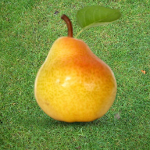
\includegraphics[width=1cm, height=1cm]{../img/poire.png}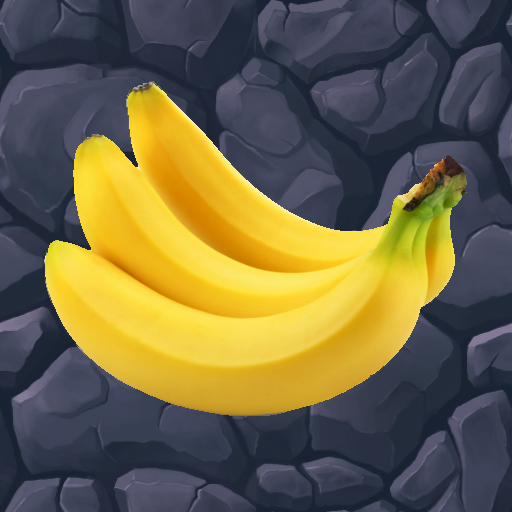
\includegraphics[width=1cm, height=1cm]{../img/banane.png}
\includegraphics[width=1cm, height=1cm]{../img/cerise.png}
\end{frame}


\section{Conclusion}
\subsection{Possibilités d'améliorations}
\begin{frame}
\frametitle{\insertsubsection}
\framesubtitle{\insertsection}
\begin{itemize}
\item L'IA ( elle peut toujours être améliorée )
\item Un mode multijoueur en réseau
\item Un changement de la taille de la grille et la possibilité de la rendre rectangulaire
\item Un système de trophées pour récompenser les joueurs
\end{itemize}

\end{frame}
\subsection{Que nous a apportez ce projet}
\begin{frame}
\frametitle{\insertsubsection}
\framesubtitle{\insertsection}
A l'aide de se projet nous avons appris à travailler en équipe, à nous entraider essayant partageant au maximum nos connaissances et en ne laissant jamais un membre du groupe avec ses problêmes mais en essayant de l'aider au mieux.\\
Nous avons aussi appris à utiliser GitHub afin de mieux coordonner nos travaux et de tous pouvoir intervenir librement sur le projet.\\
Ce projet nous a aussi permi de voir que notre organisation peut être encore améliorer afin d'être encore plus efficace.

\end{frame}

\begin{frame}
\begin{center}
	Merci de votre attention
\end{center}
\end{frame}

\end{document}